\documentclass[convert=false,border=1pt]{standalone}
\usepackage{array,tabularx}
\usepackage{float}
\usepackage{graphicx}
\usepackage{verbatim}
\usepackage{textcomp}
\usepackage{tikz}
\usepackage{pgfplots}
\usetikzlibrary{shapes,arrows,math}
\usepackage[europeanresistors,americaninductors,RPvoltages]{circuitikz}
\pgfplotsset{width=10cm,compat=1.9}

\begin{document}

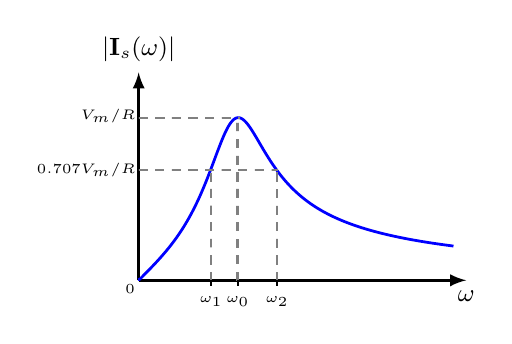
\begin{tikzpicture}[xscale=0.8, yscale=0.8]
    \draw[-latex,line width=1pt] (0,0) -- (5.2,0) node[below] {\small $\omega$};
    \draw[-latex,line width=1pt] (0,0) -- (0,3.3) node[above] {\small $|\mathbf{I}_s(\omega)|$};

%f(t)

    \draw[xscale=1,yscale=1,domain=-0.01:5,variable=\x,blue,line width=1.0pt,samples=200,opacity=1] 
    plot({\x},{1/sqrt(0.15+(0.4*\x-1/(1*\x))^2)});
    \draw[xscale=1,yscale=1,domain=0:2.58,variable=\y,gray,line width=0.8pt,samples=500,opacity=1,dashed] 
    plot({1.57},{\y});
    \draw[xscale=1,yscale=1,domain=0:1.7,variable=\y,gray,line width=0.8pt,samples=500,opacity=1,dashed] 
    plot({1.15},{\y});
    \draw[xscale=1,yscale=1,domain=0:2.2,variable=\x,gray,line width=0.8pt,samples=500,opacity=1,dashed] 
    plot({\x},{1.75});
	\draw[xscale=1,yscale=1,domain=0:1.74,variable=\y,gray,line width=0.8pt,samples=500,opacity=1,dashed] 
    plot({2.2},{\y});    
	\draw[xscale=1,yscale=1,domain=0:1.6,variable=\x,gray,line width=0.8pt,samples=500,opacity=1,dashed] 
    plot({\x},{2.58});    
    
    
    
    %Eje x tikz       
    \draw [line width = 0.7pt](1.575,0) -- (1.575,-0.09) node[below] {\tiny $\omega_0$};   
    \draw [line width = 0.7pt](1.15,0) -- (1.15,-0.09) node[below] {\tiny $\omega_1$};      
    \draw [line width = 0.7pt](2.2,0) -- (2.2,-0.09) node[below] {\tiny $\omega_2$};
    \draw [line width = 0.7pt](0.1,0.1) -- (0.1,0.1) node[below left] {\tiny $0$};      
    
    %Eje y tikz
    \draw node[left] at (0.1,2.6) {\tiny $V_m/R$};
    \draw node[left] at (0.1,1.75) {\tiny $0.707V_m/R$};
    
  \end{tikzpicture}

\end{document}